% Scaffold only. No result in this file is real until produced by code in this
% repository. Placeholder numbers are written as \TODO{} so they cannot be
% mistaken for measurements.
\documentclass[journal]{IEEEtran}

\usepackage{amsmath,amssymb}
\usepackage{booktabs}
\usepackage{graphicx}
\usepackage{xcolor}
\newcommand{\TODO}[1]{\textcolor{red}{[TODO: #1]}}

\begin{document}

\title{Measuring Watermark--Detector Interference: Controls, Score
Attenuation, and Checkpoint Dependence}

\author{\IEEEauthorblockN{Hardik\IEEEauthorrefmark{1}\IEEEauthorrefmark{2} and Yuv Jindal\IEEEauthorrefmark{2}}
\IEEEauthorblockA{\IEEEauthorrefmark{1}Dept.\ of Computer Science, Indian Institute of Technology Patna, India}
\IEEEauthorblockA{\IEEEauthorrefmark{2}Dept.\ of Computer Science and Engineering, Vivekananda Institute of Professional Studies -- TC, India}}

\maketitle

\begin{abstract}
Prior work reports that embedding a provenance watermark can \emph{harm} a
passive synthetic-image detector inspecting the same pixels. That claim has a
confound: any imperceptible perturbation shifts a detector trained on clean
images, so degradation after marking need not be watermark-specific. We
introduce a control the prior literature does not apply --- a payload-free
perturbation matched per image to the watermark's own PSNR --- and re-measure
the effect on $20{,}000$ held-out images under hypotheses fixed before the
data was scored.

The control reverses the expected conclusion. On an EfficientNet-B6
detector, the degradation attributed to watermarking belongs to the control:
matched-PSNR noise attenuates the detector's log-odds evidence toward zero by
$\approx 16\%$ (slope $0.83$--$0.85$), while watermarking leaves it
essentially intact (slope $0.97$--$0.99$). We then test whether this
attenuation is a property of detection or of one checkpoint, by repeating the
measurement on a second, provenance-disclosed detector matched to the first on
baseline AUC on the same $8{,}000$ images. \textbf{The asymmetry does not
replicate and its sign reverses}, closing off a weak-detector explanation: the
effect is checkpoint-dependent, not a general property of passive detection.

What generalises past this dataset is structural: attenuation is a monotone
rescaling and is exactly invisible to AUC while it still degrades calibration;
a mean-shift statistic cannot distinguish attenuation from translation, but a
slope estimate can. In support: the tested robust watermark's payload survives
a face-replacement-scale splice at bit error rate $0.0000$, and a
detector-floor precondition found five of six public checkpoints operating at
chance, one advertising $98.70\%$ accuracy at $\mathrm{AUC}=0.54$ in use.
\end{abstract}

\begin{IEEEkeywords}
digital watermarking, deepfake detection, image forensics, provenance,
score calibration, AUC, checkpoint generalisation, adversarial robustness,
pre-registration
\end{IEEEkeywords}

\section{Introduction}

Two defences against synthetic media are converging in deployment. Proactive
provenance marking embeds a signal at creation time so origin can be verified
later; passive detection infers manipulation from residual synthesis
artefacts. Both are computed from the same pixels, so they are not
independent: Wu et al.~\cite{wu2024watermarksbugs} report that watermarking
models built for genuine images can \emph{harm} a deployed detector, because
watermark signals overlap the forgery signals detection relies on; the same
pathology is reported independently in audio~\cite{muller2026watermarkshortcut}.
If that holds generally, a detector's score distribution shifting on marked
media invalidates any decision threshold calibrated on unmarked media.

That argument has a load-bearing confound: a detector trained on clean images
responds to \emph{any} imperceptible perturbation, so degradation after
marking need not implicate the watermark's structure. No prior work in this
space separates the two. We do, with a payload-free perturbation matched per
image to the watermark's own PSNR, reporting every interference quantity net
of that arm, with a detector-floor precondition and a gate threshold fixed
before scoring.

Our pre-registered gate returned a null on ranking. Auditing why turned the
result over: the watermark contributed almost nothing to the quantity we had
also examined, and the \emph{control} carried the effect --- not as a shift,
but as an attenuation of the detector's evidence toward zero. Attenuation with
near-zero intercept is monotone and therefore invisible to AUC by
construction, which is why a ranking gate returned a null while a real effect
was present.

That corrected mechanism then failed its own replication. Every number above
came from one third-party checkpoint with undisclosed training data, which
makes ``attenuation is a property of detection'' and ``attenuation is a
property of this model'' observationally identical. We built a second
detector with disclosed provenance --- a frozen ImageNet ResNet-18 with a
logistic head fitted only on the training split --- and repeated the
measurement. The asymmetry did not appear (\S\ref{sec:replication}): the
payload-free arm attenuated \emph{less} than the watermarked one, on images
where the two detectors are matched to within $0.003$ AUC. Sensitivity to
matched-PSNR noise is therefore a fact about a checkpoint, not about passive
detection, and the field's usual apparatus --- one detector, no control, AUC
as the outcome --- cannot see either confound.

This paper's spine is four results in sequence: a control that overturns an
attribution, the structural reason the field's standard metric misses it, a
replication that bounds how far the mechanism generalises, and what survives
that bounding. Three supporting measurements are reported as such, not as
independent claims of equal weight.

\begin{enumerate}
  \item \textbf{A control that changes the sign of the conclusion.} Every
        interference quantity is reported net of a payload-free perturbation
        matched per image to the watermark's own PSNR. Without it, our own
        headline number would have read as watermark-induced degradation that
        in fact belongs to the control.
  \item \textbf{The right estimand is a slope.} A mean-shift statistic cannot
        distinguish attenuation from translation; attenuation with near-zero
        intercept is \emph{exactly} invisible to AUC because it is monotone
        (verified by unit test), which is why a ranking gate can return a
        null while a real effect is present.
  \item \textbf{A replication failure that bounds the claim}
        (\S\ref{sec:replication}). On EfficientNet-B6, matched-PSNR noise
        attenuates evidence by $\approx 16\%$ while watermarking does not; on
        a second, provenance-disclosed detector matched to within $0.003$ AUC
        on the same images, the asymmetry vanishes and reverses. Two detectors
        establish checkpoint-dependence, not which population of detectors
        exhibits the effect, and we claim no more.
  \item \textbf{Supporting measurements.} The tested robust watermark survives
        a face-replacement-scale splice at BER $0.0000$
        (\S\ref{sec:provenance-inert}); attenuation degrades a well-specified
        calibrator's ECE $4$--$5\times$ but does not reliably move decisions
        (\S\ref{sec:calibration}); and a floor check caught five of six public
        checkpoints at chance, one advertising $98.70\%$ accuracy.
\end{enumerate}

\section{Related Work}
\label{sec:related}

\textbf{Proactive watermarking.} A substantial line of work embeds a mark at
creation time to establish provenance, increasingly unifying provenance with
detection or localisation~\cite{wu2026allinone,zeng2026lava}. Our concern is
orthogonal: what embedding a mark does to a passive detector inspecting the
same pixels, treating watermark strength (one hand-crafted, one learned
scheme) as an experimental axis rather than proposing a new one.

A larger line of work responds to the failure mode we measure in
\S\ref{sec:provenance-inert}: robust, spatially redundant watermarks survive
localised tampering for the same reason they survive benign processing, which
makes them poor at answering ``was this edited''. Semi-fragile and
separable-decoder schemes break that coupling --- SepMark's two decoders
(robust Tracer, fragile Detector)~\cite{wu2023sepmark}, fractal- and
landmark-derived constructions~\cite{wang2025fractalforensics,wang2024lampmark},
image-bit-steganography reframings~\cite{zhang2024editguard,zhang2025omniguard},
and wavelet/graph, diffusion-conditioned, and GIF-specific
embeddings~\cite{he2025waveguard,sun2025diffmark,che2026gifguard} all exist
because the failure mode is understood well enough to design around. A second,
orthogonal failure surface is diffusion-based regeneration, which degrades a
payload through global stochastic transformation rather than local
editing~\cite{zhang2024zodiac,ni2025diffusionbreaks,qi2026editingaway}. Two
different mechanisms --- regeneration and splicing --- converge on the same
conclusion about robust watermarking's limits.

\textbf{Passive detection.} Reported accuracy transfers poorly once inputs are
perturbed~\cite{hopf2026ntire}; watermark robustness has been benchmarked in
the same spirit~\cite{an2024waves}. Our E0 result is a sharp instance: a
detector advertising $98.70\%$ accuracy operates at chance on a distribution
it was not tuned for.

\textbf{Interference.} The premise this work tests is Wu et
al.'s~\cite{wu2024watermarksbugs} argument that watermarks devised for genuine
images ``may harm the deployed Deepfake detectors ... since the watermarks are
prone to overlap with the forgery signals used for detection'', answered with
AdvMark, fine-tuning the watermark itself. The same pathology is reported
independently in audio~\cite{muller2026watermarkshortcut}. Guo et
al.~\cite{guo2024passiveorwatermark} benchmark passive against watermark-based
detection head-to-head but never combine them, so whether marking degrades the
passive detectors being benchmarked is not asked. Two gaps follow, which this
paper addresses: no prior interference result controls for generic
perturbation sensitivity, and none is tested under a pre-registered null.
Consequences for a fused decision rule remain open; our corpus cannot settle
that (Limitations).

\section{Method}
\label{sec:method}
\subsection{Provenance evidence as a likelihood ratio}
Let the recovered payload contain $k_e$ bit errors out of $L$. Under intact
provenance, errors are channel noise, $k_e \sim \mathrm{Bin}(L, p_0)$; under no
valid provenance the recovered bits are uninformative, $k_e \sim
\mathrm{Bin}(L, 1/2)$. The provenance log-likelihood ratio is
\begin{equation}
  z_P = L\log 2 + k_e \log p_0 + (L - k_e)\log(1-p_0),
  \label{eq:zp}
\end{equation}
with $p_0$ estimated on a held-out clean-transform calibration set. $z_P$ is in
log-odds units and is defined only when a mark is present.

\subsection{Interference and the evidence-transfer estimator}
For watermark scheme $s$ and class $y$,
\begin{align}
  \Delta_\mu(s,y)   &= \mathbb{E}[V \mid W{=}1, S{=}s, Y{=}y] - \mathbb{E}[V \mid W{=}0, Y{=}y],\\
  \Delta_{\mathrm{AUC}}(s) &= \mathrm{AUC}(V; W{=}1, S{=}s) - \mathrm{AUC}(V; W{=}0).
\end{align}
The attenuation analyses of \S\ref{sec:confirm}--\ref{sec:replication} add one
estimator: for each arm $s$ we fit $v_s = a_s + b_s v_{\text{clean}}$ by OLS,
\emph{per arm and per detector separately}, since the question is whether an
arm's slope differs from $1$, not whether arms differ from each other by
assumption. Every fit is \emph{paired} on the same image. Confidence intervals
on $b_s$ and on slope differences are $95\%$ percentile bootstrap over images
(resampling an image moves all its arms together), $800$--$2{,}000$ resamples
depending on the analysis. Where two detectors' slopes are compared
(\S\ref{sec:replication}), both fits use the identical image set, so a
difference in $b_s$ cannot be an artefact of a difference in sample.

\subsection{Fusion and abstention}
\begin{equation}
  \hat{y} = \sigma\!\left(\beta_0 + \beta_1 z_P + \beta_2 V + \beta_3 W
            + \beta_4 (W\!\cdot\!V)\right).
  \label{eq:fusion}
\end{equation}
The independence assumption implicit in naive fusion forces $\beta_4 = 0$;
$\beta_4 \neq 0$ measures interference inside the decision rule. With costs
$c_{FN}, c_{FP}, c_R$, Chow's rule~\cite{chow1970reject} gives
\begin{equation}
  \tau_{lo} = \frac{c_R}{c_{FN}}, \qquad
  \tau_{hi} = 1 - \frac{c_R}{c_{FP}},
  \label{eq:chow}
\end{equation}
valid iff $c_R/c_{FN} + c_R/c_{FP} < 1$, and optimal only if $\hat{y}$ is
calibrated --- the dependency this paper is about.

\section{Experimental Setup}
\label{sec:setup}

\textbf{Data.} A public corpus of StyleGAN-generated faces against real
photographs, balanced by class: whole-image synthesis, \emph{not} face-swap or
reenactment, hence ``synthetic-image detection'' throughout (Limitations
states the cost of that substitution). The exploratory pass used $150{+}150$
images; the confirmatory analysis scores $20{,}000$ held-out images across
five arms (clean, two schemes, two matched nulls), and \S\ref{sec:replication}
adds a second detector over $8{,}000$ of them --- $140{,}000$ detector
evaluations total, released as raw per-image scores. Splits are stratified at
the image level (no identity metadata), so confidence intervals are
sample-level bootstraps.

\textbf{Watermarks.} Two schemes spanning the hand-crafted/learned divide,
pretrained: DWT-DCT-SVD (transform-domain) and RivaGAN (learned
encoder/decoder), both at a $32$-bit payload. Measured imperceptibility:
$36.9$\,dB / $0.967$ SSIM and $40.2$\,dB / $0.983$ respectively. For every
image and scheme we additionally generate a payload-free perturbation
binary-searched to match \emph{that image's} PSNR to within $0.5$\,dB; all
interference quantities are net of this arm. PSNR matching is not spectral
matching, so the control bounds generic perturbation sensitivity without
fully isolating watermark structure.

\textbf{Detectors.} Six public checkpoints were screened; one, an
EfficientNet-B6, clears the floor of \S\ref{sec:e0}, used zero-shot with raw
logit difference $V=\ell_{\text{fake}}-\ell_{\text{real}}$ rather than softmax
confidence. Its training data is undisclosed, so results are within-model,
within-image deltas. Because one undisclosed checkpoint cannot separate a
property of detection from a property of a model, we add a second detector we
train ourselves: a frozen ImageNet ResNet-18 feature extractor ($512$-d) with
an $\ell_2$-regularised logistic head fitted on the training split alone.
Validation and test are untouched by construction, and the head is
deliberately linear --- the most architecturally distant thing that still
clears the floor, so a shared effect is evidence of generality and a divergent
one is evidence against it.

\textbf{Protocol.} The detector floor, the gate threshold on
$\Delta\mathrm{AUC}_{net}$, and the fallback framing for a null were fixed
before scoring. Every number below is produced by released code from a single
configuration file.

\section{Results}

\subsection{Detector floor check (E0)}
\label{sec:e0}

A detector near chance makes $\Delta$AUC a measurement of noise. We screened
six public checkpoints; \textbf{five operate at chance}:

\begin{table}[t]
\centering
\caption{Baseline AUC of every screened checkpoint.}
\label{tab:e0}
\footnotesize
\begin{tabular}{lrl}
\toprule
Checkpoint & Baseline AUC & Status \\
\midrule
EfficientNet-B6 (\texttt{Skullly}) & 0.8952 & clears floor \\
ViT (\texttt{Wvolf}) & 0.5365 & chance; card claims $98.70\%$ \\
\texttt{DaMsTaR/Detecto} & 0.5365 & chance \\
\texttt{prithivMLmods/v2} & 0.5299 & chance \\
\texttt{dima806} & 0.5296 & chance \\
\texttt{Hemg} & 0.4576 & below chance \\
\bottomrule
\end{tabular}
\end{table}

Two checkpoints agree to four decimal places across 300 images, suggesting one
is a re-upload of the other, so the pool of genuinely independent public
detectors is smaller than a hub search implies. The gap between a card's
$98.70\%$ and $\mathrm{AUC}=0.54$ in use is not a rounding error; a floor
check is what stands between such a checkpoint and a table of confident noise.
It also bounds this study --- only one public detector clears the floor --- so
rather than state that as a limitation we removed it by training a second,
disclosed detector (\S\ref{sec:replication}).

\subsection{Confirmatory result ($n = 20{,}000$)}
\label{sec:confirm}

Chronology, as recorded in a git-timestamped pre-registration: (1) an
exploratory pass at $n{=}300$ on \emph{test} found no effect on ranking; (2)
repairing an unrelated defect exposed $\Delta\mu_{net}$, previously
unexamined, on a 36-image slice --- it was large; (3) because that observation
was post-hoc, we wrote a second pre-registration committing H1/H2/H3 and their
analysis code before scoring further; (4) confirmatory hypotheses were tested
on \emph{validation} ($n{=}20{,}000$), untouched by (1)--(2). One disclosed
deviation: at $2\%$ of the run, a pipeline-verification script incidentally
exposed interim values consistent with H1/H2; the run was not altered in
response, and the full log is released with the code.

\begin{table}[t]
\centering
\caption{Confirmatory pre-registered tests, net of the control arm.}
\label{tab:confirm}
\footnotesize
\begin{tabular}{lcc}
\toprule
Scheme & $\Delta\mu_{net}$ (H1) & $\Delta\mathrm{AUC}_{net}$ (H2) \\
\midrule
DWT-DCT-SVD & $\mathbf{+0.837}$ [$+0.807,+0.867$] & $+0.0049$ [$+0.0032,+0.0066$] \\
RivaGAN     & $\mathbf{+1.353}$ [$+1.317,+1.387$] & $-0.0051$ [$-0.0071,-0.0033$] \\
\bottomrule
\end{tabular}
\end{table}

Both tests pass, but \textbf{$\Delta\mu_{net}$ is the wrong estimand}: an
audit shows the watermark contributes almost nothing for DWT-DCT-SVD
($-0.009$ watermark$-$clean vs.\ $-0.846$ null$-$clean; net $+0.837$ is the
control falling). Nor is it a location shift --- it ranges $-0.36$ to $+2.28$
across clean-score quintiles. Regressing each arm on the clean score:

\begin{table}[t]
\centering
\caption{Evidence-transfer regression, EfficientNet-B6.}
\label{tab:transfer}
\footnotesize
\begin{tabular}{lrr}
\toprule
Arm & slope $b$ & intercept $a$ \\
\midrule
DWT-DCT-SVD & $0.968$ & $+0.125$ \\
null (PSNR-matched) & $\mathbf{0.834}$ & $-0.158$ \\
RivaGAN & $0.990$ & $+0.649$ \\
null (PSNR-matched) & $\mathbf{0.850}$ & $-0.125$ \\
\bottomrule
\end{tabular}
\end{table}

\textbf{The mechanism is attenuation}: random perturbation shrinks this
detector's log-odds evidence toward zero by $\approx 16\%$ ($b\approx0.84$,
$a\approx0$) while watermarking leaves it intact ($b\approx0.97$--$0.99$).
\S\ref{sec:replication} shows this is checkpoint-specific; the consequences
below are not, since they are properties of the statistics. First,
\textbf{attenuation is invisible to AUC by construction} (monotone rescaling,
verified by unit test), which is why our AUC gate returned a null while a real
effect was present. Second, \textbf{attenuation is precisely what breaks
calibration}, shrinking log-odds toward zero and changing the
score-to-posterior mapping. Effect sizes (clean-score sd $7.04$): net effects
of $0.12$--$0.19$ sd, paired Cohen's $d_z$ of $0.38$/$0.55$ --- moderate, and
class-dependent: the null arm erodes evidence on manipulated images roughly
$3\times$ more than on real ones.

\subsection{Replication on a provenance-disclosed detector}
\label{sec:replication}

One undisclosed checkpoint cannot separate ``attenuation is a property of
detection'' from ``attenuation is a property of this model''. We built a
detector with disclosed provenance --- frozen ImageNet ResNet-18, logistic
head on \emph{training} alone --- and refit the regression on the same
$8{,}000$ images restricted to the identical set both detectors scored:

\begin{table}[t]
\centering
\caption{Cross-detector slope comparison, identical images, 800-resample bootstrap.}
\label{tab:replication}
\footnotesize
\setlength{\tabcolsep}{3pt}
\begin{tabular}{llccc}
\toprule
Detector & Scheme & wm $b$ [95\% CI] & null $b$ [95\% CI] & null$-$wm \\
\midrule
EffNet-B6 & DWT & $0.966$ [$.962,.971$] & $\mathbf{0.832}$ [$.825,.839$] & $\mathbf{-.134}$ \\
EffNet-B6 & Riva & $0.987$ [$.983,.992$] & $\mathbf{0.848}$ [$.841,.856$] & $\mathbf{-.139}$ \\
ResNet-18 & DWT & $0.956$ [$.951,.962$] & $0.971$ [$.967,.974$] & $\mathbf{+.014}$ \\
ResNet-18 & Riva & $0.949$ [$.943,.954$] & $0.976$ [$.972,.979$] & $\mathbf{+.027}$ \\
\bottomrule
\end{tabular}
\end{table}

\textbf{The asymmetry does not replicate, and its sign reverses}: on the
disclosed detector the null attenuates \emph{less} than the watermark, against
$16\%$ more on EfficientNet-B6, with tight, disjoint intervals.

\begin{figure}[t]
\centering
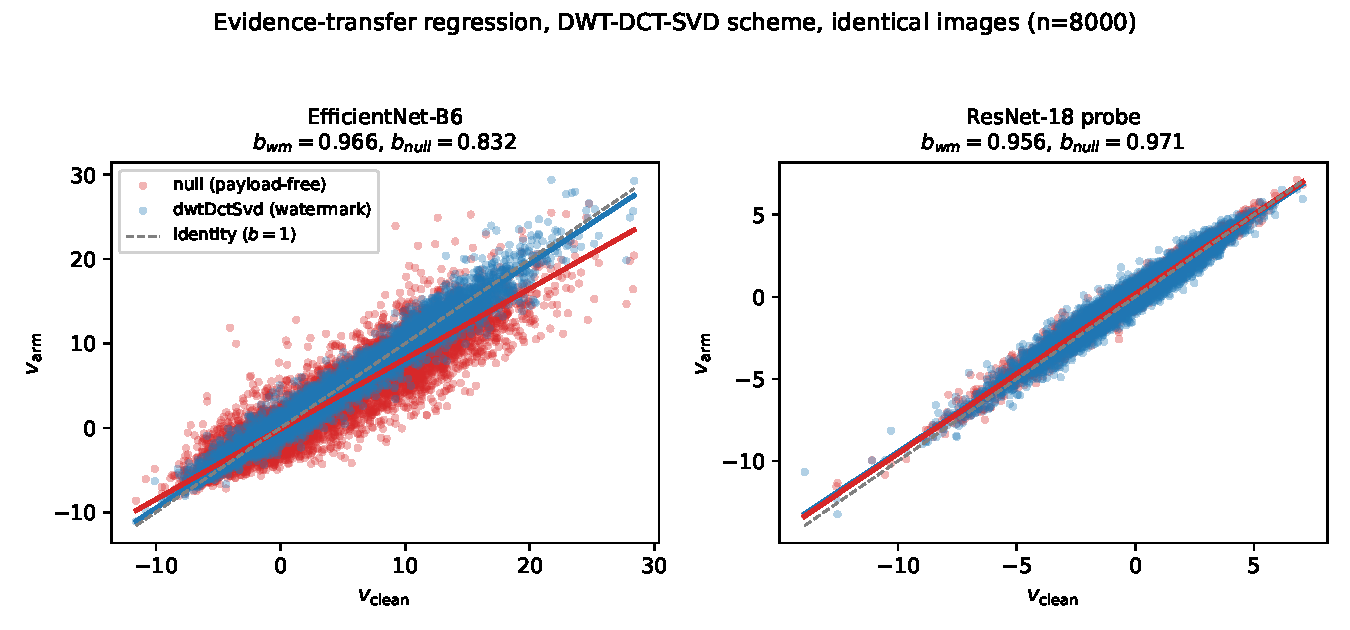
\includegraphics[width=\linewidth]{figures/fig_replication}
\caption{Evidence-transfer regression on the same $8{,}000$ images, DWT-DCT-SVD
scheme. EfficientNet-B6 (left) shows the null arm (red) pulled below identity
while the watermark (blue) tracks it; the ResNet-18 probe (right) shows the
opposite ordering.}
\label{fig:replication}
\end{figure}

The escape that a linear probe is too weak to show the effect is closed by
matched baseline AUC on the same images: $0.8703$ (EfficientNet-B6) vs.\
$0.8725$ (ResNet-18 probe), moving near-identically under every arm. What
differs is how the score \emph{distribution} moves --- exactly what the
regression measures and AUC cannot see. We therefore withdraw ``imperceptible
noise attenuates evidence while watermarking does not'' as a general claim:
EfficientNet-B6's sensitivity is a fact about that model (plausibly training
augmentation, or its $528{\times}528$ processing resolution vs.\ the probe's
$224{\times}224$). The control arm is only more strongly motivated by this:
without it, a study would report the null's $-0.846$ shift as the watermark's;
with it but one detector --- every interference paper we are aware of, and
this one until this section --- it would report a checkpoint artefact as a
property of detection. The structural results ($\Delta\mu$ conflates
attenuation with translation; AUC is exactly blind to it) are analytic and
unaffected by replication.

\subsection{Robust watermarks cannot see localised manipulation}
\label{sec:provenance-inert}

The source framework routes ``is the watermark present, and has it been
altered?'' into detection. We supplied the missing manipulation step ---
watermarking an authentic image, \emph{then} splicing a donor region in with
Poisson blending --- and measured BER against manipulated area:

\begin{figure}[t]
\centering
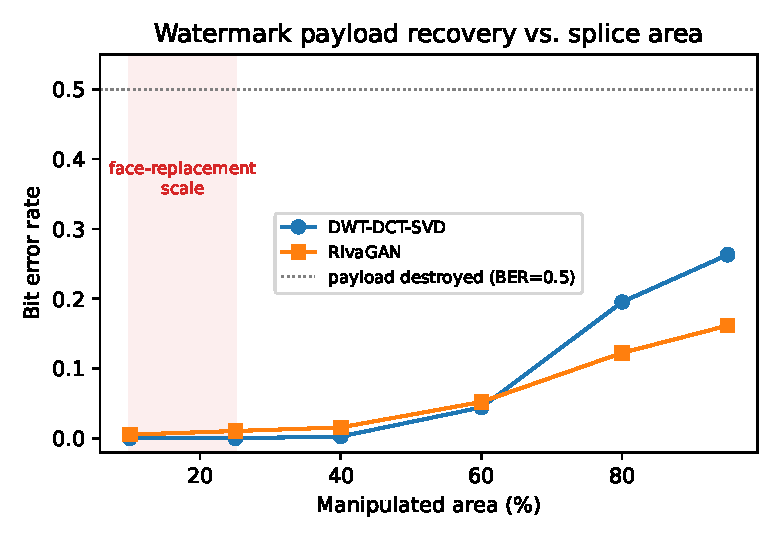
\includegraphics[width=0.9\linewidth]{figures/fig_ber_area}
\caption{BER of the recovered payload vs.\ spliced area. The shaded band is
realistic face-replacement coverage; both curves are near-zero across it.}
\label{fig:ber_area}
\end{figure}

At $10$--$25\%$ coverage --- what a face replacement costs --- the payload
survives \emph{intact} (BER $0.0000$); obliterating $95\%$ still leaves BER at
$0.26$, far from the destruction threshold of $0.5$. This is a property of
robust watermarking, not our corpus: the redundancy that survives JPEG,
resizing and re-encoding is what survives a region being replaced. We do not
claim this beyond the scheme and mechanism tested, though it is generic enough
that a robust, spatially redundant scheme behaving otherwise would surprise
us. Consequently, a fused decision rule over this channel combines one
informative signal with a constant --- the planned fusion comparison is
ill-posed here, not merely underpowered, which is why \S\ref{sec:related}'s
semi-fragile schemes exist as a response to exactly this failure. The
crossover sits at $40$--$60\%$ manipulated area, far outside realistic face
manipulation.

\subsection{Calibration under attenuation}
\label{sec:calibration}

Attenuation degrades calibration, not just rank; we measure this with ECE
under Platt and isotonic calibration~\cite{guo2017calibration}, fit on the
\emph{clean} half of a calibration split and frozen before evaluation:

\begin{table}[t]
\centering
\caption{Expected calibration error by arm and calibrator.}
\label{tab:calibration}
\footnotesize
\begin{tabular}{lccc}
\toprule
Arm & Platt ECE & Isotonic ECE & slope vs.\ clean \\
\midrule
clean            & $0.1273$ & $\mathbf{0.0094}$ & $1.000$ \\
DWT-DCT-SVD      & $0.1228$ & $0.0154$ & $0.968$ \\
RivaGAN          & $0.1353$ & $0.0290$ & $0.990$ \\
null[DWT]        & $0.0958$ & $\mathbf{0.0492}$ & $0.834$ \\
null[RivaGAN]    & $0.1009$ & $\mathbf{0.0456}$ & $0.850$ \\
\bottomrule
\end{tabular}
\end{table}

\begin{figure}[t]
\centering
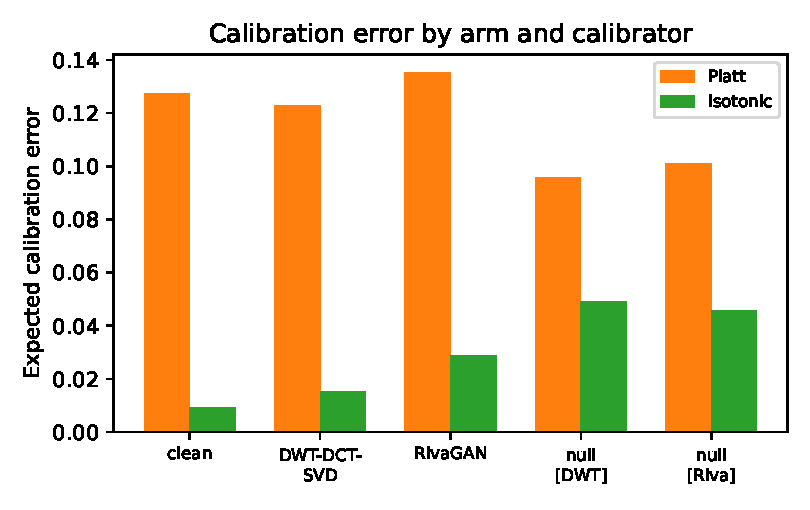
\includegraphics[width=\linewidth]{figures/fig_calibration}
\caption{ECE by arm under each calibrator. Isotonic shows attenuation
degrading calibration; Platt shows the opposite, resolved by its badly
misspecified clean-arm baseline ($0.1273$, $13\times$ isotonic's).}
\label{fig:calibration}
\end{figure}

Isotonic shows attenuation degrading ECE $4$--$5\times$ over clean while
watermarking degrades it far less; Platt shows the null arms
\emph{improving}, which we resolve rather than cherry-pick: Platt's clean-arm
ECE is already $13\times$ isotonic's (raw logits span $-11.6$ to $+36.8$,
sd$=7.04$), so its baseline is broken before any perturbation, and attenuation
happens to partially cancel that misspecification. The claim survives for
calibration \emph{quality} and fails for decision \emph{risk}: isotonic DRD is
$0.0055$ (clean), $0.0145$/$0.0054$ (nulls) --- small and inconsistent in
direction. Attenuation reaches the probability estimates without reliably
moving decisions at these costs.

\subsection{Why the fusion comparison is not reported, and transform robustness}
\label{sec:e4e5}

The planned fusion comparison (F0--F5, with/without an interaction term) is
not reported: \S\ref{sec:provenance-inert} shows the provenance channel
constant under manipulation, so any recovered $\beta_4$ would describe
sampling noise, not signal. We instead report a different fusion question ---
whether $\beta_4$ responds to a standard transform on otherwise unmanipulated
images --- at reduced scale, flagged as a first look: $n{=}400$ (120/280
split, held-out \emph{test}, disjoint from validation), EfficientNet-B6, seven
transforms, \emph{no bootstrap interval computed}.

\begin{table}[t]
\centering
\caption{Transform robustness, F0 (no interaction) vs.\ F4 (with it), n=400.}
\label{tab:e4}
\footnotesize
\setlength{\tabcolsep}{3pt}
\begin{tabular}{lrrrrr}
\toprule
Transform & F0 AUC & F0 DRD & F4 AUC & F4 DRD & F4 $\beta_4$ \\
\midrule
JPEG(90)     & 0.899 & 0.006 & 0.897 & 0.008 & $+0.004$ \\
JPEG(70)     & 0.776 & 0.003 & 0.819 & 0.005 & $-0.022$ \\
JPEG(50)     & 0.721 & 0.001 & 0.794 & 0.005 & $+0.038$ \\
Resize(0.75) & 0.743 & 0.003 & 0.825 & 0.008 & $+0.048$ \\
Resize(0.5)  & 0.710 & 0.001 & 0.825 & $\mathbf{0.050}$ & $\mathbf{+0.221}$ \\
Bright($+20\%$) & 0.909 & 0.034 & 0.909 & 0.031 & $+0.056$ \\
Bright($-20\%$) & 0.841 & 0.003 & 0.848 & 0.006 & $-0.072$ \\
\bottomrule
\end{tabular}
\end{table}

\begin{figure}[t]
\centering
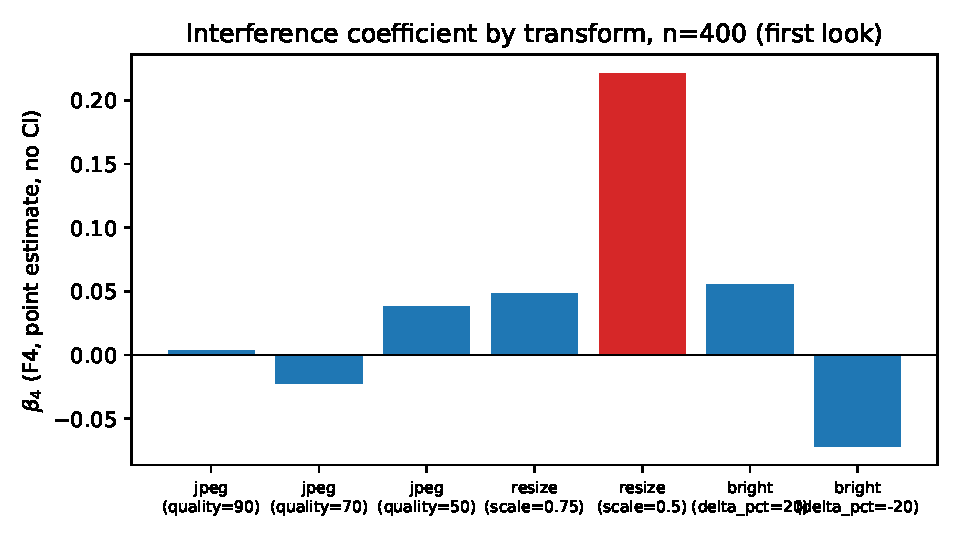
\includegraphics[width=\linewidth]{figures/fig_e4_beta4}
\caption{$\beta_4$ per transform (F4, n=280, no CI). Resize-to-$0.5\times$
(shaded) is $3$--$6\times$ every other condition and is flagged, not claimed.}
\label{fig:e4_beta4}
\end{figure}

F0 and F4 AUC move together under compression/resize --- the detector's own
fragility, not a watermark effect. $\beta_4$ stays small ($<0.08$) for six of
seven transforms; resize-to-$0.5\times$ is an outlier ($\beta_4=+0.221$, DRD
$0.050$). At $n{=}280$ with no interval, this is flagged for a CI-backed
rerun, not claimed. The $\rho$ sweep (fusion fit once on calibration,
evaluated on watermarked-fraction mixtures) found AUC/ECE/DRD essentially flat
across $\rho\in\{0.05,0.25,0.5,1.0\}$ for both schemes:

\begin{figure}[t]
\centering
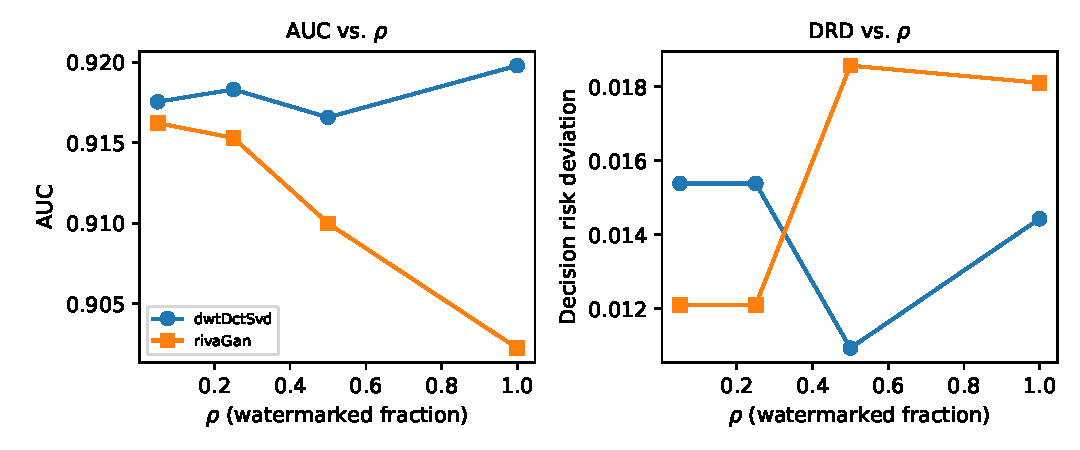
\includegraphics[width=\linewidth]{figures/fig_rho_sweep}
\caption{AUC and decision-risk deviation vs.\ watermarked fraction $\rho$,
model F4. Both are flat, consistent with the provenance channel's weak
contribution elsewhere in this paper.}
\label{fig:rho_sweep}
\end{figure}

--- consistent with the provenance channel's weak contribution throughout: if
it does not move the outcome at $\rho{=}1$, its prevalence will not matter
either.

\section{Limitations}

\textbf{Provenance channel inertness, measured not assumed.} We supplied the
manipulation step the source framework presupposes and measured the channel
still inert (\S\ref{sec:provenance-inert}) --- a finding, not a corpus
artefact. Our splice is faithful to the provenance mechanics but not to a
learned face swap's detector-facing realism, so claims concern localised
tampering generally, not modern face-swap detectability specifically.

\textbf{Statistical power.} The $n{=}300$ exploratory pass has AUC standard
error $\approx0.03$, larger than the effects measured, so its null means
``undetectable at this size''. Confirmatory and replication analyses
($n{=}20{,}000$/$8{,}000$) do not have this problem; reported intervals, not
point estimates, bound excluded effect sizes.

\textbf{Synthesis type.} Whole-image GAN synthesis vs.\ real photographs, not
face-swap/reenactment as in standard benchmarks~\cite{rossler2019faceforensics};
detectors keying on generator fingerprints need not generalise to different
manipulation traces.

\textbf{Detector provenance and count.} The strong detector's training data is
undisclosed (mitigated by within-model, within-image deltas); the disclosed
detector is a linear probe on generic features, not an engineered detector.
Two detectors establish non-universality, not which population of detectors
exhibits the effect --- that needs a panel, and \S\ref{sec:e0} shows floor-
clearing detectors are the scarce resource.

\textbf{Other.} Interference is measured zero-shot; a task-trained detector is
untested. Decision thresholds use an assumed cost triple and swept, not
measured, $\rho$.

\section{Discussion}

\textbf{What a null does and does not mean.} We did not detect
\cite{wu2024watermarksbugs}'s effect in our setting, which is a boundary
condition, not a refutation: their detectors are trained for the manipulation
family they evaluate and their images are manipulated \emph{after} marking,
so watermark and forgery signals coexist as their argument describes. Ours are
zero-shot detectors on whole-image synthesis marked after the fact.

\textbf{Ranking vs.\ calibration.} $\Delta\mathrm{AUC}$ is silent on
translation, which leaves ranking untouched while invalidating a posterior
calibrated on unmarked media --- exactly our own pre-registered gate's
asymmetry ($\Delta\mathrm{AUC}_{net}$ tested; a calibration-centred thesis
needs $\Delta\mu_{net}$). Any reading of the latter here is post-hoc; the
correct response is a fresh pre-registration, not a reinterpretation.

\textbf{One checkpoint is not a detector.} \S\ref{sec:replication}'s
replication failure is the result we would have preferred to avoid and the
one most worth reporting: a $16\%$ attenuation, sign-reversed on a model
matched to $0.003$ AUC. The claim is not that our probe is the right second
detector --- it is a weak one --- but that a difference on one checkpoint is
not yet a finding, and the cheapest fix (a frozen backbone with a linear head)
is within any paper's budget.

\textbf{Detector floors deserve to be standard.} A precondition check cost
almost nothing and caught a checkpoint at chance while advertising $98.70\%$.
Any study measuring a difference in detector behaviour inherits the
assumption that the detector behaves at all.

\section{Conclusion}

We set out to measure whether provenance watermarking interferes with passive
synthetic-image detection; the defensible answer is narrower than the one we
started toward. Against a PSNR-matched control on $20{,}000$ images, an
EfficientNet-B6 detector's evidence is attenuated $\approx16\%$ by
imperceptible noise and left intact by watermarking --- and against a second,
disclosed detector matched to $0.003$ AUC, that asymmetry reverses. Two
detectors show the effect is checkpoint-dependent, not which population it
belongs to; we claim only the former, and only because we ran both the
control arm and the second model, neither standard practice here.

What generalises is structural: a mean-shift statistic conflates attenuation
with translation, and AUC is exactly blind to monotone attenuation, so gating
on $\Delta\mathrm{AUC}$ while measuring with $\Delta\mu$ can be simultaneously
wrong about the mechanism and unable to see it. The tested robust watermark
carries no information about the manipulation it is meant to flag (BER
$0.0000$ at realistic coverage), so fusion over it combines one source with a
constant. A floor check caught five of six public detectors at chance, one
advertising $98.70\%$ accuracy --- a precondition for trusting the above.

The useful reading is not that interference is absent, but that the apparatus
commonly used to look for it --- one checkpoint, no control, AUC as the
outcome --- cannot tell an effect from its control, a model from its
architecture family, or a calibration-relevant change from a null.

{\footnotesize
\bibliographystyle{IEEEtran}
\bibliography{refs}}

\end{document}
